
\section{Enruteamiento Multicast}

El multicast proporciona un medio de comunicación de punto a multipunto,
en el que el origen envía mensajes a varios destinos.

Para realizar la comunicación de punto de uno a muchos la forma más
sencilla es enviar el mensaje desde la fuente a cada uno de los destinos
de forma separada e independiente, es lo que se llama múltiples Unicast.

A diferencia de varios unicast, multicast es una forma más eficiente
para implementar la comunicación uno a muchos, haciendo mejor uso
de los recursos de la red.

Por lo tanto, multicast es considerada como la tecnología clave para
apoyar y soportar las demandas de las aplicaciones de uso intensivo
de ancho de banda de punto a multipunto, tales como televisión de
alta definición (HDTV), videoconferencia, video demanda (VOD), distribución
de documentos multimedia, aprendizaje interactivo a distancia, subastas
en vivo, juegos distribuidos, óptica storage área networks (O-SAN),
computación distribuida, replicación de base de datos, y así sucesivamente\cite{zhou2005optical}.

En el problema de enrutamiento multicast se puede dar dos tipos de
traficos: Establecimiento estatico donde los requerimientos de demandas
se conocen a priori, es decir, el problema de diseño de la red se
resuelve de ante mano y Establecimiento Dinamico los requerimientos
de demandas van iniciando de acuerdo a las necesidades en este tipo
de establecimiento uno de los objetivos principales es la de minimizar
los bloqueos.

En las figuras \prettyref{fig:Multiples-unicast-versus} se muestra
un ejemplo de las diferentes formas de realizar multidifusión por
ejemplo en la figura \prettyref{fig:Multiples-unicast} se observa
que para enviar un mensaje a los tres destinos se necesita tres canales
diferentes, y en la figura \prettyref{fig:Multicast} se puede apreciar
que para el mensaje al mismo número de destinos se requiere solo un
canal.

\begin{figure}[H]
\subfloat[Multiples\foreignlanguage{english}{ unicast \label{fig:Multiples-unicast}}]{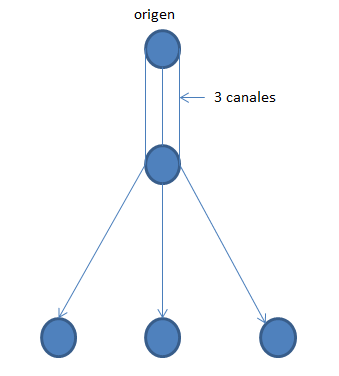
\includegraphics[scale=0.45]{04_multicast/imagenes/multicasVariosUnicast}}\subfloat[\selectlanguage{english}%
Multicast \label{fig:Multicast}\selectlanguage{spanish}%
]{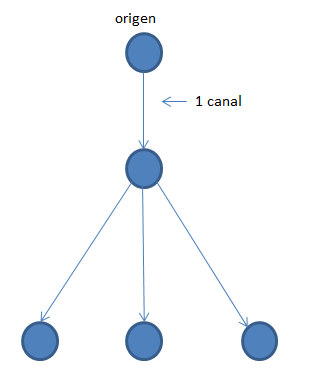
\includegraphics[scale=0.45]{04_multicast/imagenes/multicasUnCanal}}\caption{Multiples unicast versus multicast \foreignlanguage{english}{\label{fig:Multiples-unicast-versus}}}
\end{figure}


En la literatura, multicast óptico se refiere a la realización de
la multidifusión directamente en la capa óptica de red.

Para la realizar multidifusión en las redes WDM se pueden utilizar
dos mecanismos de construcción de red: a) Multidifusión a través de
redes Broadcast-and-select y b) multidifusión a través de redes wavelength-routed
\cite{zhou2005optical}.

Una red Broadcast-and-select cada nodo transmite datos de multidifusión
utilizando una simple longitud de onda. Los nodos destinos seleccionaban
la información que necesitaban sintonizando algunas de las longitudes
de onda. Este tipo de redes presentaba una topología del tipo estrella
\cite{diegopinto2011}.

Una red óptica Wavelength-routed adopta una topología malla y cada
nodo de la red está equipado con un conmutador fotonico dinámicamente
configurable, es decir, con un conector óptico cruzado (OXC).

Los componentes claves para llevar a cabo la multidifusión basado
en wavelength-routed son los divisores de luz (Splitting) y los OXC. 

Un Splitting es un dispositivo óptico pasivo que tiene la capacidad
inherente de dividir una señal de luz de entrada en varias salidas
como se puede observar en la figura \prettyref{fig:Splitting-que-divide}

\begin{figure}[H]
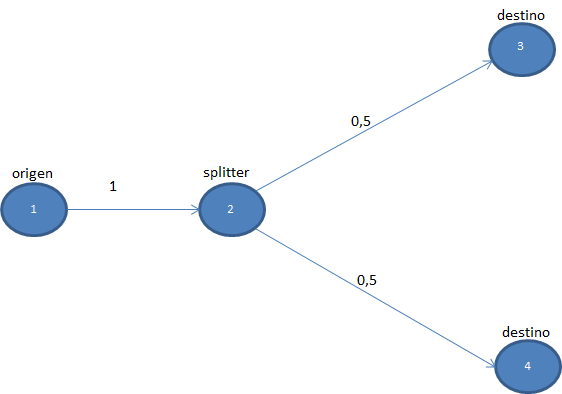
\includegraphics[scale=0.45]{04_multicast/imagenes/Splitter}\caption{Splitting que divide la señal que proviene del nodo 1 a los destinos
3 y 4. \label{fig:Splitting-que-divide}}
\end{figure}


La multidifusión en la capa óptica puede alcanzar alta velocidad de
procesamiento al eliminar el cuello de botella de procesamiento electrónico.

Un OXC que tiene la capacidad de dividir la luz se conoce como capacidad
de multidifusión OXC (MC-OXC). 

Una arquitectura tipica OXC capaz de realizar multidifusion (MC-OXC)
fue propuesto en\cite{hu1998multicasting}, se basa en switches splitter-and-delivery
(SAD), como se puede apreciar en \ref{fig:SAD-based-MC-OXC.}. En
un switch SAD NxN, en cada puerto de entrada, la señal de luz se divide
primeramente en N salidas, cada uno de los cuales es cambiando a un
puerto fijo de salida o descartados por el conmutador optico. En esta
arqutectura SAD-basado en MC-OXC, cada señal de luz de entrada se
puede cambiar a ninguno, unom multiples o a todos los puertos de salida.
Por lo tanto, la arquitectura SAD es estrictamente sin bloqueo.



\begin{figure}[H]
\subfloat[Un MC-OXC N × N . \label{fig:NxNMCOXC}]{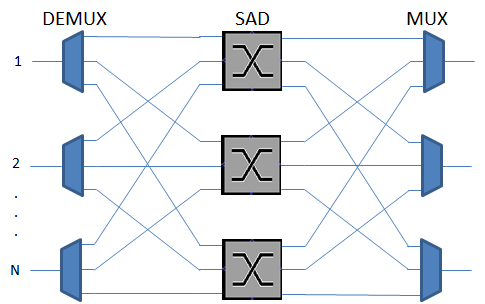
\includegraphics[scale=0.4]{04_multicast/imagenes/NxN-MC-OXC_PP}}\subfloat[Un switch SAD N × N . \label{fig:NxNSAD}]{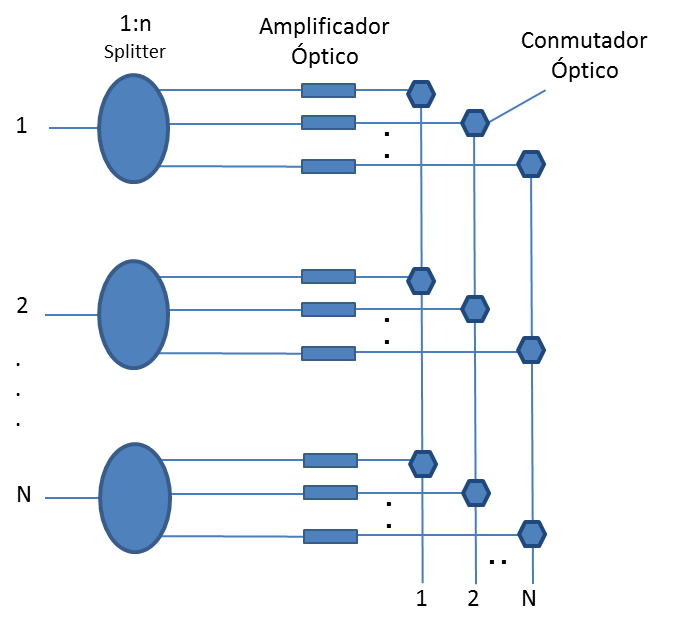
\includegraphics[scale=0.45]{04_multicast/imagenes/NxN-SADswitchPP}}\caption{SAD-based MC-OXC. \label{fig:SAD-based-MC-OXC.}}
\end{figure}


Si todos los nodos de la red tienen capacidad de multidifusión la
red es full light splitting, y si en una red algunos nodos no cuentan
con capacidad de multidifusión y otros nodos si la red es light spare
splitting.

En este trabajo asumimos que no tenemos conversor de longitud de onda
como ya se había mencionado en la introducción y se centra en un red
\emph{light splitting}.

Los problemas de multicast óptico se pueden clasificar en: plano de
datos y plano de control \cite{rouskas2003optical} y estos problemas
se resumen en \ref{tab:Clasificacion-de-problemas}.

\begin{table*}[!t]
\begin{tabular}{|l|>{\raggedright}p{3cm}|>{\centering}p{3cm}|>{\raggedright}p{3cm}|>{\centering}p{4cm}|}
\hline 
\textbf{Bloques de contruccion} & \multicolumn{3}{c|}{\textbf{Principales problemas}} & \textbf{Principales limitaciones}\tabularnewline
\hline 
\multirow{2}{*}{Plano de Datos} & \multirow{1}{3cm}{Diseño eficiente de potencia} & \multicolumn{2}{>{\raggedright}p{5cm}|}{Perdida de potencia debido a los divisores de luz} & Perdida de potencia de la señal debido al splitting\tabularnewline
\cline{2-5} 
 & Diseño con costo efectivo & \multicolumn{2}{>{\raggedright}m{5cm}|}{Número de amplificadores ópticos y convertidores de longitud de onda} & Número de amplificadores ópticos y convertidores de longitud de onda\tabularnewline
\hline 
\multirow{9}{*}{Plano de Control} & \multirow{6}{3cm}{MC-RWA} & \multirow{4}{3cm}{Solicitud simple} & Modelo light-tree  & Número de longitudes de onda\tabularnewline
\cline{4-5} 
 &  &  & Modelo multi-drop & Capacidad de dividir la luz \tabularnewline
\cline{4-5} 
 &  &  & Modelo multi$\lambda$-light-tree & Capacidad de conversión de longitud de onda\tabularnewline
\cline{4-5} 
 &  &  & Modelo light-forest & Consideración de energía\tabularnewline
\cline{3-5} 
 &  & \multirow{2}{3cm}{Multiples solicitudes} & Trafico estatico & Rendimiendo por bloqueo\tabularnewline
\cline{4-5} 
 &  &  & Trafico Dinamico & \tabularnewline
\cline{2-5} 
 & \multicolumn{3}{l|}{Evaluación del desempeño de multicast} & Límites de longitud de onda, modelo de bloqueo\tabularnewline
\cline{2-5} 
 & \multicolumn{3}{l|}{Proteccion de trafico multicast} & Fallo de enlace único\tabularnewline
\cline{2-5} 
 & \multicolumn{3}{l|}{Trafico multicast grooming} & Solicitud de conexión de baja velocidad\tabularnewline
\hline 
\end{tabular}\caption{Clasificacion de problemas de multicast optico con wavelength-routed
en redes WDM \foreignlanguage{english}{\label{tab:Clasificacion-de-problemas}}}
\end{table*}


En el \textbf{plano de datos}, el problema fundamental es el estudio
de la arquitectura MC-OXC cuya optimización de dicho plano esta principalmente
limitada por los parámetros de hardware.

En el \textbf{plano de control}, el problema es el enrutamiento multicast
y asignación de longitud de onda (MC-RWA). Este estrecho acoplamiento
entre encaminamiento y asignación de longitud de onda surge con el
fin de establecer una conexión óptica, donde se trata tanto el encaminamiento
(seleccionar la ruta adecuada) y la asignación de longitud de onda.

El diseño eficiente de potencia se refiere a diseñar una red en el
cual se requiera un mínimo número de splitting en el MC-OXC con mínimos
efectos en el rendimiento de una red con bloqueos.

El diseño con costo efectivo para diseñar una red de manera a disminuir
el costo que acarrea utilizar conversores de longitudes de onda para
evitar los bloqueos y diseñar el uso de amplificadores ópticos que
se utilizan de manera a solucionar los problemas que traen consigo
los splitting al perder potencia de señal y problemas de atenuación,
Sin embargo, la complejidad de fabricación de los amplificadores en
OXC puede ser muy alto. En consecuencia, el costo-rendimiento trade-off
debe ser cuidadosamente considerado en la construcción de la MC-OXC.

MC-RWA para multicast simple para diseñar una red para satisfacer
una solicitud multicast única. Algunas métricas utilizadas para calcular
el costo son: costo del uso de una longitud de onda en un enlace dado,
costo de conversión de longitud de onda, costo de un dividir la luz,
retardo de la transmisión (delay) y el retardo de la conversión de
la longitud de onda de entrada a la de salida.

Multicast simple con el modelo light-tree: se diseña el árbol dada
la solicitud multicast simple en una red con capacidad full de splitting
(full light splitting capability) pero sin conversores de longitud
de onda.

Multicast simple - modelo multi-drop: Se diseña la red con diferentes
longitudes de onda designadas a cada destino que se pueden dividir
en el camino para alcanzar los destinos con igual asignación de longitud
de onda. Se pueden hacer múltiples caminos y subconjuntos de destinos
con igual longitud de onda. De un nodo origen puede salir diferentes
tipos de longitud de onda para una solicitud multicast simple única.
Sin capacidad de conversión de longitud de onda.

Multicast simple - multiʎ-light-tree:se diseña el árbol multicast
en una red con capacidad full de splitting (full light splitting capability)
y capacidad de conversión de longitud de onda. Un arbol de luz puede
tener varios caminos con diferentes longitudes de onda, es decir,
una solicitud puede tener diferentes longitudes de onda al salir del
arbol.

Multicast simple - modelo light-forest: diseñar la red con la solicitud
multicast en una red con algunos nodos multicast-capable (MC) y otros
nodos multicast-incapable (MI). Es decir, en una red sparse splitting.

MC-RWA para multicast múltiple: diseñar una red para satisfacer múltiples
solicitudes multicast.

Multicast múltiple - tráfico estático: diseñar la red para un conjunto
de solicitudes estáticas que permanecen en un periodo de tiempo largo,
por lo tanto el tráfico debe calcularse fuera de línea.

Multicast múltiple - tráfico dinámico: diseñar la red para solicitudes
vienen uno a uno de forma aleatoria.

Evaluación del desempeño de multicast: para evaluar el desempeño de
un multicast óptica en una red wavelength-routed, existen dos indicadores
principales que son: el número de longitudes de onda utilizadas y
el rendimiento por bloqueo.

Protección de tráfico multicast: problemas de protección y restauración
se han estudiado de manera amplia en un escenario de solicitudes punto
a punto. Sin embargo, el estudio del mismo para solicitudes punto
a multipunto no se ha estudiado de la misma manera para redes de malla.

Trafico multicast grooming: diseñar la red cuando el requerimiento
de ancho de banda supera la capacidad del canal.

Para una solicitud point-to-point (punto a punto, unicast), aparece
el termino \textbf{light-path} (camino de luz), es decir, point-to-point
all-optical wavelength channel que puede abarcar múltiples enlaces
de fibra.

Para una solicitud de multidifusión, el concepto de light-path se
extiende a\textbf{ light-tree} (árbol de luz), que se refiere a point-to-multipoint
all-optical wavelength channel (punto a multipunto todo óptico en
una canal de longitud de onda).

Los retos de MC-RWA se encuentran en dos principales aspectos, en
primer lugar, el problema de punto a punto RWA \cite{zang2000review}en
diversos escenarios se reduce a menudo a problemas del tipo NP-Completo.
Dado un problema MC-RWA puede considerarse como un caso más general
de problema RWA, y es mucho más difícil encontrar soluciones óptimas
para MC-RWA (que es el problema también tratado en este trabajo).
En segundo lugar, como el splitting es introducido en la multidifusión,
diferentes combinaciones de capacidad de splitting y capacidad de
conversión hacen que el problema sea aún más sofisticado. En conclusión
el problema de MC-RWA no solo debe enfrentar los problemas que debe
enfrentar punto a punto RWA sino también los problemas que acarrea
la introducción del splitting , amplificadores de luz para mitigar
la perdida de potencia por división de luz.
